% =============================================================================
%  DesignWear — System Architecture (deep technical reference)
%  Compile with:  pdflatex DesignWear-Architecture.tex   (run twice for ToC)
%  Requires a TeX distribution with TikZ (TeX Live / MiKTeX).
% =============================================================================
\documentclass[11pt,a4paper]{report}

\usepackage[margin=2.2cm]{geometry}
\usepackage{tikz}
\usepackage{listings}
\usepackage{xcolor}
\usepackage{enumitem}
\usepackage{booktabs}
\usepackage{array}
\usepackage{longtable}
\usepackage{fancyhdr}
\usepackage[hidelinks]{hyperref}
\usetikzlibrary{positioning, arrows.meta, shapes.geometric, fit, backgrounds, calc}

% ---- Brand palette ----------------------------------------------------------
\definecolor{dwink}{HTML}{1F2430}
\definecolor{dwblue}{HTML}{2C5F8A}
\definecolor{dwgreen}{HTML}{1D9E75}
\definecolor{dworange}{HTML}{D8743A}
\definecolor{dwpurple}{HTML}{6B4FA0}
\definecolor{dwgray}{HTML}{5F5E5A}
\definecolor{dwyellow}{HTML}{C9962B}

% ---- TikZ component styles ---------------------------------------------------
\tikzset{
  comp/.style={rectangle, rounded corners=2.5pt, draw=dwblue, fill=dwblue!8,
    line width=0.6pt, align=center, font=\small\sffamily, inner sep=4pt,
    minimum height=11mm, text width=27mm},
  store/.style={cylinder, shape border rotate=90, aspect=0.28, draw=dwgreen,
    fill=dwgreen!12, line width=0.6pt, align=center, font=\footnotesize\sffamily,
    inner sep=2pt, minimum height=14mm, text width=20mm},
  ext/.style={rectangle, rounded corners=2pt, draw=dworange, fill=dworange!10,
    line width=0.6pt, align=center, font=\footnotesize\sffamily, inner sep=4pt,
    minimum height=9mm, text width=22mm},
  layer/.style={rectangle, rounded corners=2pt, draw=dwpurple!80, fill=dwpurple!7,
    line width=0.6pt, align=center, font=\small\sffamily, inner sep=5pt,
    minimum height=10mm, text width=0.82\linewidth},
  grp/.style={rectangle, rounded corners=3pt, draw=dwgray!45, fill=dwgray!5,
    line width=0.5pt, inner sep=6pt, align=center},
  note/.style={rectangle, draw=dwgray!40, fill=dwyellow!10, font=\scriptsize\sffamily,
    align=left, inner sep=4pt, rounded corners=2pt, text width=46mm},
  flow/.style={-{Stealth[length=2mm]}, line width=0.7pt, dwink},
  biflow/.style={{Stealth[length=2mm]}-{Stealth[length=2mm]}, line width=0.7pt, dwink},
  dflow/.style={-{Stealth[length=2mm]}, line width=0.7pt, dwgray, dashed},
  lbl/.style={font=\scriptsize\sffamily, fill=white, inner sep=1.5pt},
}

% ---- Listings ---------------------------------------------------------------
\lstdefinestyle{dw}{
  basicstyle=\ttfamily\footnotesize, breaklines=true, frame=single,
  rulecolor=\color{dwgray!35}, backgroundcolor=\color{dwgray!5},
  columns=fullflexible, keepspaces=true, showstringspaces=false,
  commentstyle=\color{dwgreen}, keywordstyle=\color{dwblue}\bfseries,
}
\lstset{style=dw}
\newcommand{\code}[1]{\texttt{#1}}

% ---- Headers ----------------------------------------------------------------
\pagestyle{fancy}\fancyhf{}
\fancyhead[L]{\footnotesize\sffamily DesignWear — System Architecture}
\fancyhead[R]{\footnotesize\sffamily\thepage}
\renewcommand{\headrulewidth}{0.3pt}

\title{\textbf{DesignWear}\\[4pt]\large System Architecture \& Technical Reference}
\author{Design-and-Remix Garment Commerce Platform\\Flutter $\cdot$ Next.js $\cdot$ Sanity $\cdot$ Firebase}
\date{Generated \today}

\begin{document}
\maketitle
\thispagestyle{empty}
\tableofcontents
\clearpage

% =============================================================================
\chapter{Introduction}
% =============================================================================

\section{What DesignWear is}
DesignWear is a \textbf{design-and-remix garment commerce platform}. End users browse
and buy garments, but they can also open an in-app \emph{Design Studio}, customise a
garment (front and back), and \emph{publish} their creation as a community product that
others can buy or remix. The platform therefore blends two domains:

\begin{itemize}[noitemsep]
  \item \textbf{E-commerce} --- catalogue, cart, checkout, payments, orders, inventory.
  \item \textbf{Creative community} --- a canvas design studio, remix lineage, likes,
        and creator attribution.
\end{itemize}

\section{Deployable units}
The system is composed of one client and one backend talking over a REST API, plus a
headless CMS and a runtime database.

\begin{center}\small
\begin{tabular}{@{}lll@{}}
\toprule
\textbf{Unit} & \textbf{Technology} & \textbf{Hosting}\\
\midrule
Frontend client & Flutter (web, Android, iOS, desktop) & Firebase Hosting (web)\\
Backend API     & Next.js 16 (App Router)              & Vercel\\
Headless CMS     & Sanity Studio (project \code{jh7llku7})       & Sanity Cloud\\
Runtime database & Cloud Firestore (project \code{designwear-731c9}) & Google Firebase\\
\bottomrule
\end{tabular}
\end{center}

\noindent The production API is served at
\code{https://designwear-backend.vishwamai.com/api}.

\section{Two sources of truth (by design)}
A recurring theme in this architecture is the deliberate split between \textbf{Sanity}
(the editorial source of truth for the catalogue) and \textbf{Firestore} (the
low-latency runtime store the client reads and writes). They are reconciled by a
one-way sync engine described in Chapter~\ref{ch:flow}.

% =============================================================================
\chapter{System Architecture}\label{ch:sys}
% =============================================================================

\section{Context diagram}
Figure~\ref{fig:context} shows the major components and the external services they
depend on. Solid arrows are runtime data flows; the dashed arrow is the
publish-time webhook that drives synchronisation.

\begin{figure}[h]\centering
\resizebox{\textwidth}{!}{%
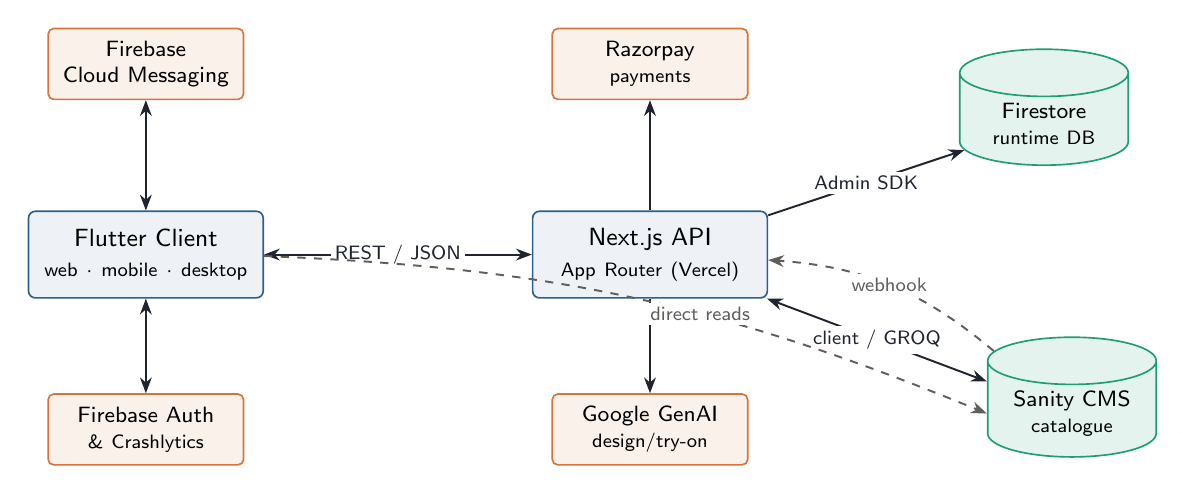
\begin{tikzpicture}[node distance=15mm and 22mm]
  \node[comp] (flutter) {Flutter Client\\\scriptsize web $\cdot$ mobile $\cdot$ desktop};
  \node[comp, right=34mm of flutter] (api) {Next.js API\\\scriptsize App Router (Vercel)};
  \node[store, above right=6mm and 30mm of api] (fs) {Firestore\\\scriptsize runtime DB};
  \node[store, below right=6mm and 30mm of api] (sanity) {Sanity CMS\\\scriptsize catalogue};

  \node[ext, above=14mm of api] (razor) {Razorpay\\\scriptsize payments};
  \node[ext, above=14mm of flutter] (fcm) {Firebase\\Cloud Messaging};
  \node[ext, below=12mm of api] (genai) {Google GenAI\\\scriptsize design/try-on};
  \node[ext, below=12mm of flutter] (auth) {Firebase Auth\\\scriptsize \& Crashlytics};

  \draw[biflow] (flutter) -- node[lbl]{REST / JSON} (api);
  \draw[flow] (api) -- node[lbl]{Admin SDK} (fs);
  \draw[biflow] (api) -- node[lbl]{client / GROQ} (sanity);
  \draw[dflow] (sanity) to[bend right=18] node[lbl]{webhook} (api);
  \draw[flow] (api) -- (razor);
  \draw[flow] (api) -- (genai);
  \draw[biflow] (flutter) -- (fcm);
  \draw[biflow] (flutter) -- (auth);
  \draw[dflow] (flutter) to[bend left=10] node[lbl,pos=0.6]{direct reads} (sanity.west);
\end{tikzpicture}}
\caption{System context: client, API, data stores, and external services.}
\label{fig:context}
\end{figure}

\section{Design principles}
\begin{description}[leftmargin=1.2cm, style=nextline]
  \item[CMS as editorial truth] Admins edit products, categories and garment templates
        in Sanity; nothing in the catalogue originates in Firestore by hand.
  \item[Firestore as runtime truth] The client reads catalogue \emph{mirrors} plus
        live commerce state (orders, carts, inventory, customers) from Firestore for speed.
  \item[Thin client, fat API] Business rules (sync, inventory transactions, payment
        verification) live in the backend; the Flutter app is presentation + orchestration.
  \item[Graceful degradation] The client falls back to bundled assets / public data and a
        ``demo mode'' when credentials or network are unavailable.
  \item[Idempotent sync] Every sync operation upserts (\code{merge}) so re-runs and
        back-fills are safe.
\end{description}

% =============================================================================
\chapter{Frontend --- Flutter}\label{ch:fe}
% =============================================================================

\section{Layered (clean) architecture}
The client follows a clean-architecture layering under \code{lib/}. Dependencies point
\emph{downward}: UI depends on use-cases, which depend on repositories, which depend on
services; models and config are shared leaves.

\begin{figure}[h]\centering
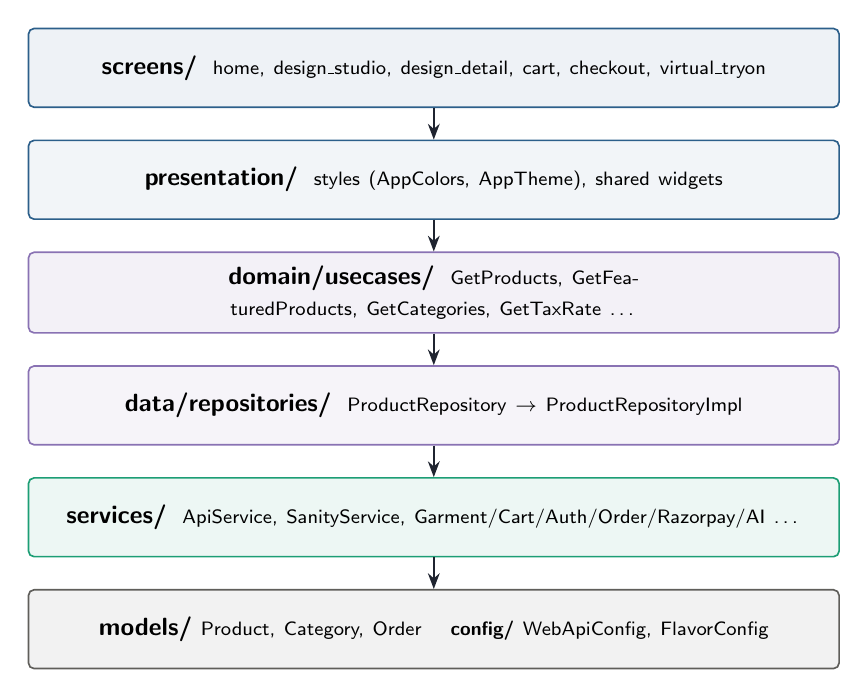
\begin{tikzpicture}[node distance=4mm]
  \node[layer, fill=dwblue!8, draw=dwblue] (screens)
    {\textbf{screens/} \;\scriptsize home, design\_studio, design\_detail, cart, checkout, virtual\_tryon};
  \node[layer, below=of screens, fill=dwblue!6, draw=dwblue]
    (pres) {\textbf{presentation/} \;\scriptsize styles (AppColors, AppTheme), shared widgets};
  \node[layer, below=of pres, fill=dwpurple!8]
    (domain) {\textbf{domain/usecases/} \;\scriptsize GetProducts, GetFeaturedProducts, GetCategories, GetTaxRate \dots};
  \node[layer, below=of domain, fill=dwpurple!6]
    (data) {\textbf{data/repositories/} \;\scriptsize ProductRepository $\rightarrow$ ProductRepositoryImpl};
  \node[layer, below=of data, fill=dwgreen!8, draw=dwgreen]
    (svc) {\textbf{services/} \;\scriptsize ApiService, SanityService, Garment/Cart/Auth/Order/Razorpay/AI \dots};
  \node[layer, below=of svc, fill=dwgray!8, draw=dwgray]
    (base) {\textbf{models/} \scriptsize Product, Category, Order \quad\textbf{config/} \scriptsize WebApiConfig, FlavorConfig};
  \draw[flow] (screens) -- (pres);
  \draw[flow] (pres) -- (domain);
  \draw[flow] (domain) -- (data);
  \draw[flow] (data) -- (svc);
  \draw[flow] (svc) -- (base);
\end{tikzpicture}
\caption{Flutter clean-architecture layers (top depends on bottom).}
\label{fig:felayers}
\end{figure}

\section{Dependency injection \& state}
Wiring happens in \code{lib/main.dart} with the \code{provider} package. A
\code{MultiProvider} constructs the repository and use-cases once, then exposes
\code{ChangeNotifier}s for cross-cutting state:

\begin{lstlisting}[caption={Provider graph (simplified)}]
Provider<ProductRepository>        -> ProductRepositoryImpl(ApiService.webApi | .sanity)
Provider<GetProductsUseCase>       -> reads ProductRepository
Provider<GetFeaturedProductsUseCase>
Provider<GetCategoriesUseCase> / GetProductByIdUseCase / GetTaxRateUseCase
ChangeNotifierProvider<CartService>(reads GetTaxRateUseCase)
ChangeNotifierProvider<AuthService>()   // .init() at startup
ChangeNotifierProvider<ThemeProvider>()
\end{lstlisting}

\section{Data-access modes}
\code{ApiService} (\code{lib/services/api\_service.dart}) has two constructors selected by
\code{WebApiConfig} in \code{lib/config/app\_config.dart}:

\begin{center}\small
\begin{tabular}{@{}lll@{}}
\toprule
\textbf{Mode} & \textbf{Constructor} & \textbf{Talks to}\\
\midrule
Web API (default) & \code{ApiService.webApi(baseUrl)} & Next.js REST (\code{WEB\_API\_BASE\_URL})\\
Direct CMS        & \code{ApiService.sanity()}        & Sanity GROQ (content reads)\\
\bottomrule
\end{tabular}
\end{center}

\noindent Configuration is injected at build time via \code{--dart-define} / web
\code{env.json}; key flags are \code{USE\_WEB\_API} and \code{WEB\_API\_BASE\_URL}.

\section{Notable services}
{\small
\begin{longtable}{@{}p{4.4cm}p{9.5cm}@{}}
\toprule
\textbf{Service} & \textbf{Responsibility}\\
\midrule
\endhead
\code{ApiService} & REST/GROQ client; product, category, order, tax endpoints.\\
\code{SanityService} & GROQ projections (e.g.\ product projection with preview images).\\
\code{GarmentService} & Loads garment \emph{templates} from \code{/garments} into \code{GarmentRegistry}.\\
\code{CartService} & Cart state + tax via \code{GetTaxRateUseCase} (ChangeNotifier).\\
\code{AuthService} & Auth/session lifecycle; \code{init()} at startup.\\
\code{OrderService} / \code{RazorpayService} & Order creation, Razorpay checkout (web + mobile stubs).\\
\code{AIAgentService} / \code{VirtualTryonService} & DesignBot, AI generation, virtual try-on.\\
\code{Design*Service} & History, storage (auto-save), templates for the Studio.\\
\code{LoggingService} & Structured client logging + route observer.\\
\bottomrule
\end{longtable}
}

\section{Design Studio (client side)}
The Studio (\code{lib/screens/design\_studio/}) renders a garment \emph{template} image and
lets the user place elements (text, stickers, images), tint the base colour, and switch
between \textbf{front} and \textbf{back} sides. An off-screen \code{Offstage} canvas
captures the opposite side at publish time so both previews are produced in one pass.
Garment options in the picker come from Sanity \emph{categories}; the rendered blank
comes from \code{GarmentRegistry} (Chapter~\ref{ch:feat}).

% =============================================================================
\chapter{Backend --- Next.js}\label{ch:be}
% =============================================================================

\section{Route map}
All endpoints are App-Router handlers under \code{designwear-backend/app/api/**/route.ts}.
Figure~\ref{fig:apimap} groups them by domain.

\begin{figure}[h]\centering
\resizebox{\textwidth}{!}{%
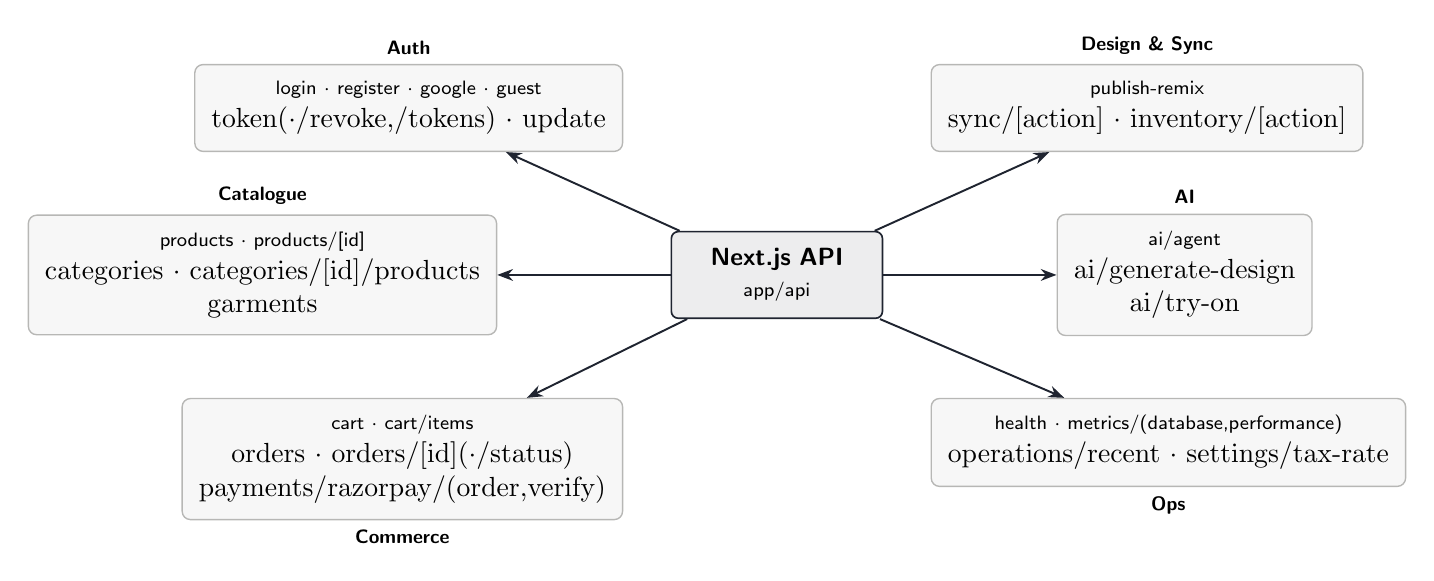
\begin{tikzpicture}[node distance=6mm]
  \node[comp, fill=dwink!8, draw=dwink, text width=24mm] (core) {\textbf{Next.js API}\\\scriptsize app/api};

  \node[grp, above left=10mm and 6mm of core, label=above:{\scriptsize\sffamily\bfseries Auth}] (auth)
    {\scriptsize\sffamily login $\cdot$ register $\cdot$ google $\cdot$ guest\\ token($\cdot$/revoke,/tokens) $\cdot$ update};
  \node[grp, left=22mm of core, label=above:{\scriptsize\sffamily\bfseries Catalogue}] (cat)
    {\scriptsize\sffamily products $\cdot$ products/[id]\\ categories $\cdot$ categories/[id]/products\\ garments};
  \node[grp, below left=10mm and 6mm of core, label=below:{\scriptsize\sffamily\bfseries Commerce}] (com)
    {\scriptsize\sffamily cart $\cdot$ cart/items\\ orders $\cdot$ orders/[id]($\cdot$/status)\\ payments/razorpay/(order,verify)};
  \node[grp, above right=10mm and 6mm of core, label=above:{\scriptsize\sffamily\bfseries Design \& Sync}] (ds)
    {\scriptsize\sffamily publish-remix\\ sync/[action] $\cdot$ inventory/[action]};
  \node[grp, right=22mm of core, label=above:{\scriptsize\sffamily\bfseries AI}] (ai)
    {\scriptsize\sffamily ai/agent\\ ai/generate-design\\ ai/try-on};
  \node[grp, below right=10mm and 6mm of core, label=below:{\scriptsize\sffamily\bfseries Ops}] (ops)
    {\scriptsize\sffamily health $\cdot$ metrics/(database,performance)\\ operations/recent $\cdot$ settings/tax-rate};

  \foreach \n in {auth,cat,com,ds,ai,ops}{\draw[flow] (core) -- (\n);}
\end{tikzpicture}}
\caption{Backend REST surface grouped by domain.}
\label{fig:apimap}
\end{figure}

\section{Server libraries}
\begin{center}\small
\begin{tabular}{@{}p{5.2cm}p{8.7cm}@{}}
\toprule
\textbf{Module} & \textbf{Role}\\
\midrule
\code{lib/config/database.ts} & Firebase Admin init from \code{FIREBASE\_SERVICE\_ACCOUNT\_KEY}; exports a lazy \code{db} (Firestore), \code{auth}, \code{messaging} via proxies; \code{firebaseReady} guard.\\
\code{lib/services/syncService.ts} & Sanity$\rightarrow$Firestore product sync, customer$\rightarrow$Sanity sync, and inventory mirror + movement logging (Ch.~\ref{ch:flow}).\\
\code{lib/utils/logger.ts} & \code{winston} structured logging.\\
\code{sanity/} & Schema types, \code{structure.ts} (Studio nav), \code{actions/PublishAndSync.ts}.\\
\bottomrule
\end{tabular}
\end{center}

\noindent Most handlers follow the same shape: guard \code{firebaseReady}; read query/body;
talk to Firestore/Sanity; return \code{NextResponse.json(\{ success, data \})}; log + 500 on error.

% =============================================================================
\chapter{Content \& Data Model}\label{ch:data}
% =============================================================================

\section{Sanity schema types}
Thirteen document types live in \code{sanity/schemaTypes/}. The \code{product} type is the
richest, organised into field groups: \emph{basic, pricing, media, studio, community, meta}.

{\small
\begin{longtable}{@{}p{3.4cm}p{10.6cm}@{}}
\toprule
\textbf{Type} & \textbf{Key fields}\\
\midrule
\endhead
\code{product} & name, slug, description, category$\rightarrow$, tags, sku, price, taxRate,
  compareAtPrice, stock, lowStockThreshold, images[], sizes, colors, customizable,
  \textbf{garmentType}, \textbf{creatorHandle}, garmentBaseColor, artText,
  remixedFromHandle/Version, likeCount, remixCount, lineage[], designJson,
  previewImage, backPreviewImage, status, featured, supplier$\rightarrow$, dbSyncStatus.\\
\code{garmentTemplate} & id, label, frontImage, backImage, supportsCollarPocket, sortOrder.\\
\code{category} & name, slug, description, image, parent$\rightarrow$.\\
\code{order} & orderNumber, customer$\rightarrow$, items[\{product,qty,size,color,price\}],
  totalAmount, status, paymentStatus, shippingAddress, orderDate, notes.\\
\code{customer} & name, email, phone, addresses[], totalOrders, totalSpent, registeredAt.\\
\code{inventoryMovement} & product$\rightarrow$, type, quantity, reason, reference, notes, performedBy, timestamp.\\
\code{supplier} & name, contactPerson, email, phone, address, website, notes.\\
\code{designTemplate} & templateId, name, description, category, thumbnail, tags, designData, active, order.\\
\code{deal} & label, originalPrice, salePrice, discountPercent, colorHex, product$\rightarrow$, image, active, expiresAt.\\
\code{homeBanner} & badge, title, subtitle, ctaLabel, ctaAction, ctaColor, image, order, active.\\
\code{categoryQuickLink} & label, iconName, colorHex, action, tabIndex, order, active.\\
\code{notificationTemplate} & name, eventType, title, body.\\
\code{systemLog} & level, category, message, details\{error,stack,metadata\}, timestamp.\\
\bottomrule
\end{longtable}
}

\section{Firestore collections (runtime)}
\begin{center}\small
\begin{tabular}{@{}p{3.2cm}p{4.0cm}p{6.6cm}@{}}
\toprule
\textbf{Collection} & \textbf{Written by} & \textbf{Notes}\\
\midrule
\code{products} & sync, publish-remix & Catalogue + community-design mirror.\\
\code{inventory} & inventory sync/backfill/adjust & One doc per \emph{stocked} product.\\
\code{inventoryMovements} & inventory sync/adjust & Append-only stock audit.\\
\code{orders} & checkout & Razorpay/Stripe orders.\\
\code{carts} & cart API & Server-side carts.\\
\code{customers} & auth / customer sync & Profiles (mirrored to Sanity).\\
\code{operationLogs} & syncService & Sync operation audit.\\
\bottomrule
\end{tabular}
\end{center}

\section{The two kinds of ``product''}
A single \code{product} type backs two very different objects. The distinguishing signal
is \code{creatorHandle}.

\begin{center}\small
\begin{tabular}{@{}lll@{}}
\toprule
 & \textbf{Catalogue product} & \textbf{Designed garment}\\
\midrule
Origin & admin in Sanity / \code{POST /products} & Design Studio $\rightarrow$ \code{publish-remix}\\
\code{creatorHandle} & absent & present (required)\\
Stock model & tracked in \code{inventory} & print-on-demand (not stocked)\\
Imagery & \code{images[]} & canvas \code{previewImage} (+ back)\\
\bottomrule
\end{tabular}
\end{center}

\begin{figure}[h]\centering
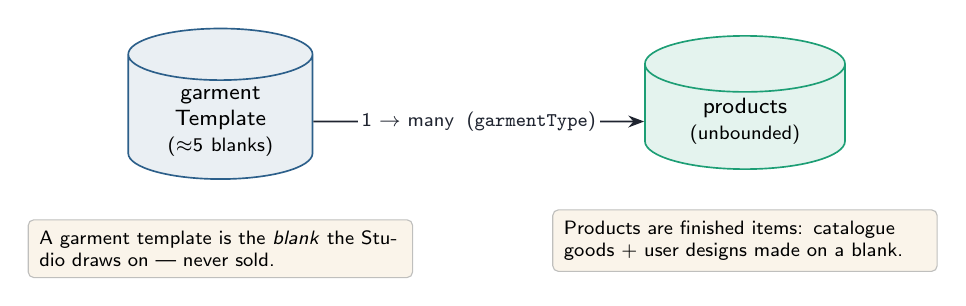
\begin{tikzpicture}[node distance=8mm]
  \node[store, fill=dwblue!10, draw=dwblue, text width=22mm] (gt) {garment\\Template\\\scriptsize ($\approx$5 blanks)};
  \node[store, right=42mm of gt, text width=24mm] (prod) {products\\\scriptsize (unbounded)};
  \draw[flow] (gt) -- node[lbl]{1 $\rightarrow$ many \;(\code{garmentType})} (prod);
  \node[note, below=5mm of gt] {A garment template is the \emph{blank} the Studio draws on --- never sold.};
  \node[note, below=5mm of prod] {Products are finished items: catalogue goods + user designs made on a blank.};
\end{tikzpicture}
\caption{Garment templates vs.\ products: one blank powers many products.}
\label{fig:gtvsp}
\end{figure}

% =============================================================================
\chapter{Data Flow \& Synchronisation}\label{ch:flow}
% =============================================================================

\section{Catalogue sync (Sanity $\rightarrow$ Firestore)}
When a product is published in Sanity, a webhook calls \code{POST /api/sync/webhook},
which invokes \code{syncProductToDatabase(id)}. That mirrors the product into Firestore
\emph{and} (for stocked items) upserts an inventory record.

\begin{figure}[h]\centering
\resizebox{0.96\textwidth}{!}{%
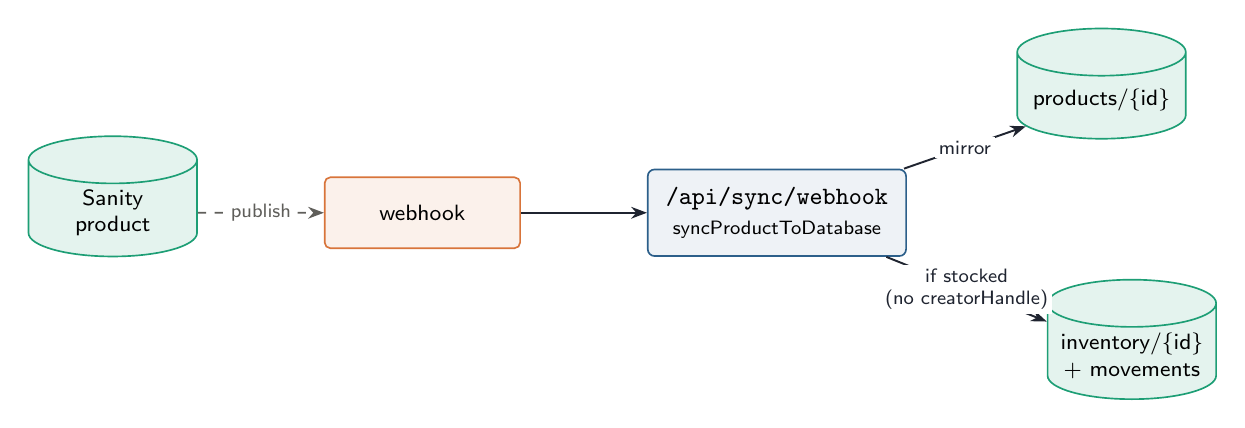
\begin{tikzpicture}[node distance=10mm and 16mm]
  \node[store] (san) {Sanity\\product};
  \node[ext, right=of san] (hook) {webhook};
  \node[comp, right=of hook, text width=30mm] (route) {\code{/api/sync/webhook}\\\scriptsize syncProductToDatabase};
  \node[store, above right=4mm and 20mm of route] (pcol) {products/\{id\}};
  \node[store, below right=4mm and 20mm of route] (inv) {inventory/\{id\}\\+ movements};
  \draw[dflow] (san) -- node[lbl]{publish} (hook);
  \draw[flow] (hook) -- (route);
  \draw[flow] (route) -- node[lbl]{mirror} (pcol);
  \draw[flow] (route) -- node[lbl,align=center]{if stocked\\(no creatorHandle)} (inv);
\end{tikzpicture}}
\caption{Publish-time catalogue + inventory synchronisation.}
\label{fig:sync}
\end{figure}

\noindent \code{GET /api/sync/status} reports \code{pendingItems}, \code{failedItems} and
\code{lastSync}. \emph{Prerequisite:} the Sanity webhook must target the deployed
\code{/api/sync/webhook}.

\section{Design publish (Studio $\rightarrow$ product)}
Publishing a design posts the front/back canvas PNGs, the design JSON and creator
metadata. The backend uploads previews to the Sanity CDN, creates and publishes a Sanity
\code{product}, and writes a Firestore mirror with usable CDN URLs.

\begin{figure}[h]\centering
\resizebox{0.96\textwidth}{!}{%
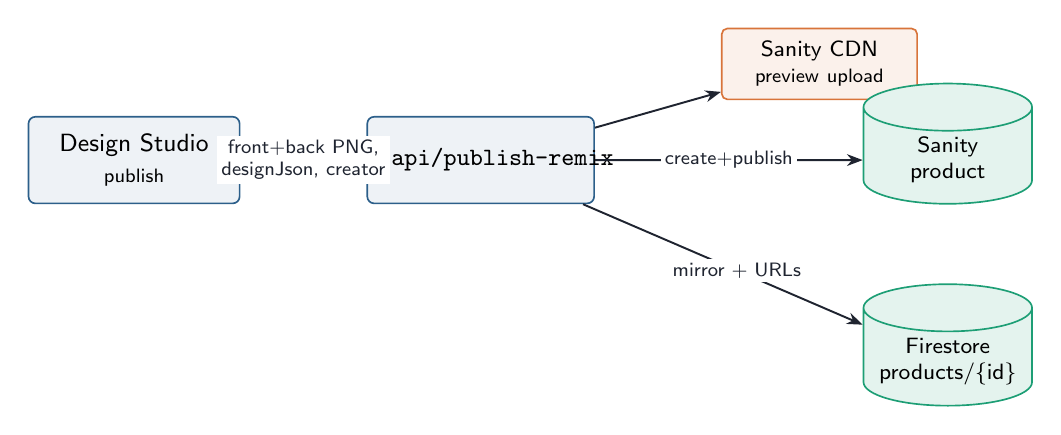
\begin{tikzpicture}[node distance=9mm and 16mm]
  \node[comp, text width=24mm] (studio) {Design Studio\\\scriptsize publish};
  \node[comp, right=of studio, text width=26mm] (pr) {\code{/api/publish-remix}};
  \node[ext, above right=2mm and 16mm of pr] (cdn) {Sanity CDN\\\scriptsize preview upload};
  \node[store, right=34mm of pr] (sdoc) {Sanity\\product};
  \node[store, below=10mm of sdoc] (fdoc) {Firestore\\products/\{id\}};
  \draw[flow] (studio) -- node[lbl,align=center]{front+back PNG,\\designJson, creator} (pr);
  \draw[flow] (pr) -- (cdn);
  \draw[flow] (pr) -- node[lbl]{create+publish} (sdoc);
  \draw[flow] (pr) -- node[lbl,pos=0.55]{mirror + URLs} (fdoc);
\end{tikzpicture}}
\caption{Studio publish (\code{publish-remix}) creates a linked product in both stores.}
\label{fig:remix}
\end{figure}

\section{Inventory pipeline}
Inventory is a first-class concern with two collections beyond \code{products}.
\code{upsertInventoryRecord} runs in one transaction: it writes \code{inventory/\{id\}}
and, when the stock level changed, appends an \code{inventoryMovements} audit entry.
Only \emph{stocked} products (no \code{creatorHandle}) are tracked.

\begin{figure}[h]\centering
\resizebox{0.96\textwidth}{!}{%
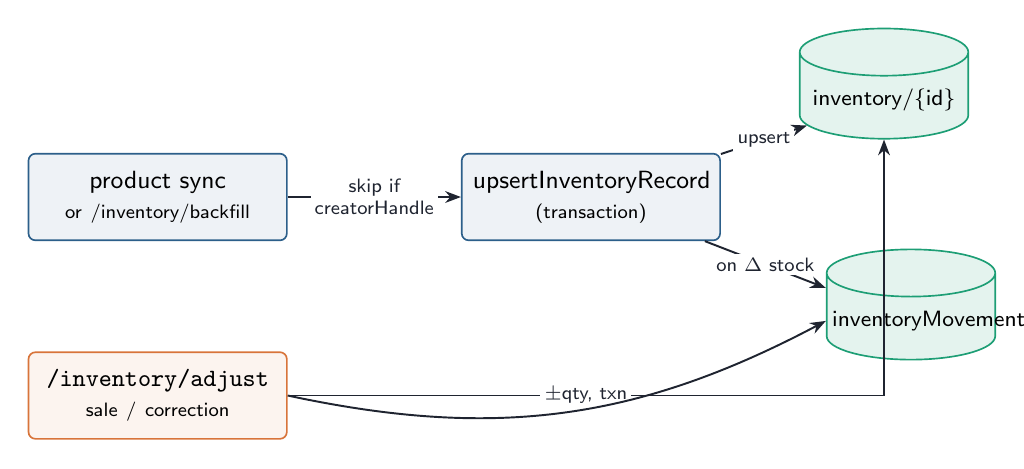
\begin{tikzpicture}[node distance=8mm and 15mm]
  \node[comp, text width=30mm] (sync) {product sync\\\scriptsize or /inventory/backfill};
  \node[comp, right=22mm of sync, text width=30mm] (up) {upsertInventoryRecord\\\scriptsize (transaction)};
  \node[store, above right=2mm and 16mm of up] (inv) {inventory/\{id\}};
  \node[store, below right=2mm and 16mm of up] (mov) {inventoryMovements};
  \node[comp, below=14mm of sync, text width=30mm, draw=dworange, fill=dworange!8] (adj)
    {\code{/inventory/adjust}\\\scriptsize sale / correction};
  \draw[flow] (sync) -- node[lbl,align=center]{skip if\\creatorHandle} (up);
  \draw[flow] (up) -- node[lbl]{upsert} (inv);
  \draw[flow] (up) -- node[lbl]{on $\Delta$ stock} (mov);
  \draw[flow] (adj) -| node[lbl,pos=0.25]{$\pm$qty, txn} (inv);
  \draw[flow] (adj.east) to[bend right=20] (mov.west);
\end{tikzpicture}}
\caption{Inventory mirror + audit; \code{adjust} performs transactional stock changes.}
\label{fig:inv}
\end{figure}

\section{Checkout}
\code{POST /api/payments/razorpay/order} creates a Razorpay order; the client completes
payment; \code{POST /api/payments/razorpay/verify} validates the
\code{razorpay\_signature}; the order is persisted in Firestore \code{orders}.
\emph{Open item:} a paid order does not yet decrement inventory (the \code{adjust}
endpoint is the intended hook).

% =============================================================================
\chapter{MCP Integration}\label{ch:mcp}
% =============================================================================

\section{Purpose}
The Model Context Protocol (MCP) lets an AI agent (Claude) operate on the live stack as
an \textbf{on-demand operations console} --- back-fills, audits, ad-hoc queries --- using
the same data the backend serves. It is \emph{not} the always-on automation path; that
remains the backend webhook (Chapter~\ref{ch:flow}).

\section{Configuration}
The project ships a committed \code{.mcp.json} at the repository root wiring two servers.
No secrets are stored: Sanity uses hosted OAuth and Firebase reuses the local CLI login.

\begin{lstlisting}[caption={.mcp.json configuration}]
{
  "mcpServers": {
    "sanity":   { "type": "http", "url": "https://mcp.sanity.io" },
    "firebase": { "command": "cmd", "args": ["/c","firebase","experimental:mcp"] }
  }
}
\end{lstlisting}

\begin{figure}[h]\centering
\resizebox{0.92\textwidth}{!}{%
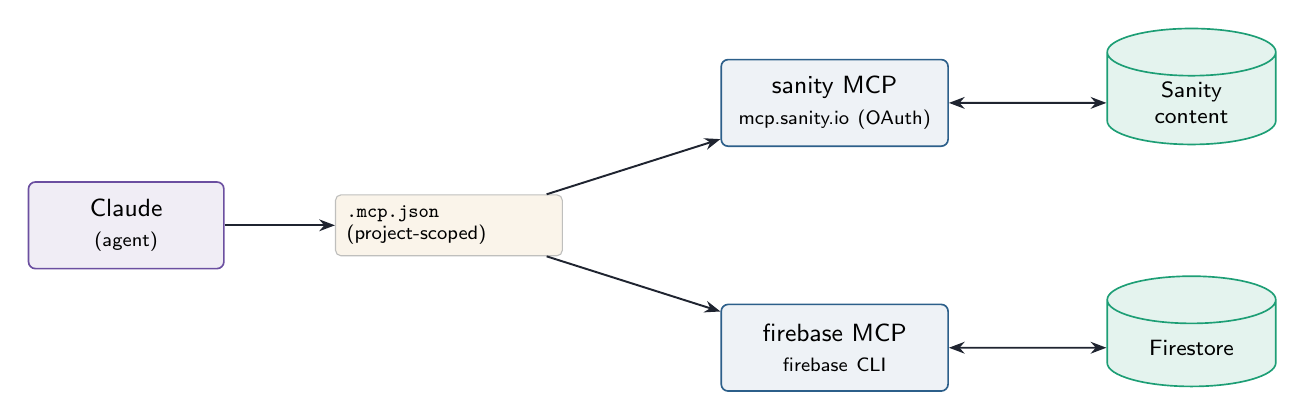
\begin{tikzpicture}[node distance=10mm and 18mm]
  \node[comp, text width=22mm, fill=dwpurple!10, draw=dwpurple] (claude) {Claude\\\scriptsize (agent)};
  \node[note, text width=26mm, right=14mm of claude] (cfg) {\code{.mcp.json}\\(project-scoped)};
  \node[comp, above right=6mm and 20mm of cfg, text width=26mm] (msan) {sanity MCP\\\scriptsize mcp.sanity.io (OAuth)};
  \node[comp, below right=6mm and 20mm of cfg, text width=26mm] (mfb) {firebase MCP\\\scriptsize firebase CLI};
  \node[store, right=20mm of msan] (san) {Sanity\\content};
  \node[store, right=20mm of mfb] (fs) {Firestore};
  \draw[flow] (claude) -- (cfg);
  \draw[flow] (cfg) -- (msan);
  \draw[flow] (cfg) -- (mfb);
  \draw[biflow] (msan) -- (san);
  \draw[biflow] (mfb) -- (fs);
\end{tikzpicture}}
\caption{MCP wiring: Claude reaches Sanity and Firestore through two servers.}
\label{fig:mcp}
\end{figure}

\section{Typical operations}
\begin{itemize}[noitemsep]
  \item ``Back-fill inventory for every product'' $\rightarrow$ \code{POST /api/inventory/backfill}
        or direct Firestore writes via the firebase MCP.
  \item ``Show low-stock items'' $\rightarrow$ query \code{inventory} where \code{status == "lowStock"}.
  \item ``Record a sale'' $\rightarrow$ \code{POST /api/inventory/adjust} with negative delta.
  \item ``Audit drift'' $\rightarrow$ diff \code{products} against \code{inventory}.
\end{itemize}

% =============================================================================
\chapter{Deployment \& Operations}\label{ch:deploy}
% =============================================================================

\section{Topology}
\begin{figure}[h]\centering
\resizebox{\textwidth}{!}{%
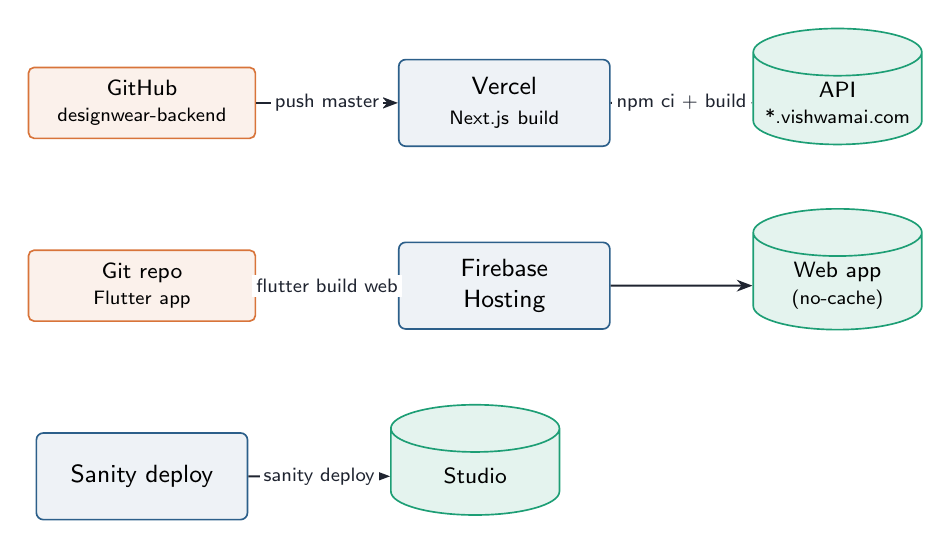
\begin{tikzpicture}[node distance=9mm and 18mm]
  \node[ext, text width=26mm] (ghb) {GitHub\\\scriptsize designwear-backend};
  \node[comp, right=of ghb, text width=24mm] (vercel) {Vercel\\\scriptsize Next.js build};
  \node[store, right=of vercel] (api) {API\\\scriptsize *.vishwamai.com};
  \node[ext, below=14mm of ghb, text width=26mm] (ghf) {Git repo\\\scriptsize Flutter app};
  \node[comp, right=of ghf, text width=24mm] (fbh) {Firebase\\Hosting};
  \node[store, right=of fbh] (web) {Web app\\\scriptsize (no-cache)};
  \node[comp, below=14mm of ghf, text width=24mm] (sanity) {Sanity deploy};
  \node[store, right=of sanity] (studio) {Studio};

  \draw[flow] (ghb) -- node[lbl]{push master} (vercel);
  \draw[flow] (vercel) -- node[lbl]{npm ci + build} (api);
  \draw[flow] (ghf) -- node[lbl]{flutter build web} (fbh);
  \draw[flow] (fbh) -- (web);
  \draw[flow] (sanity) -- node[lbl]{sanity deploy} (studio);
\end{tikzpicture}}
\caption{Deployment surfaces: backend (Vercel), web app (Firebase Hosting), Studio (Sanity).}
\label{fig:deploy}
\end{figure}

\section{Build commands}
\begin{center}\small
\begin{tabular}{@{}lll@{}}
\toprule
\textbf{Surface} & \textbf{Build} & \textbf{Install / serve}\\
\midrule
Backend & \code{next build} & \code{npm ci --legacy-peer-deps} (Vercel)\\
Web app & \code{flutter build web --release} & Firebase Hosting, \code{no-cache} headers\\
Studio  & \code{npx sanity deploy} & Sanity Cloud\\
\bottomrule
\end{tabular}
\end{center}

\section{Operational gotchas}
\begin{description}[leftmargin=0.8cm, style=nextline]
  \item[\code{npm ci} lock sync] Changing \code{package.json} (e.g.\ removing an
        \code{overrides} entry) \emph{requires} regenerating \code{package-lock.json}.
        Vercel's \code{npm ci} hard-fails on any mismatch
        (\code{Missing: undici@\dots\ from lock file}). Verify with
        \code{npm ci --legacy-peer-deps --dry-run} before pushing.
  \item[Web caching] Serve \code{main.dart.js} with \code{no-cache}; a long-cached bundle
        makes deploys appear stale.
  \item[Garment templates] The Studio falls back to a bundled blank until a
        \code{garmentTemplate} is \emph{published} with front/back images.
  \item[Sync webhook] Auto-sync only runs if the Sanity webhook targets
        \code{/api/sync/webhook}.
  \item[Known open items] paid-order $\rightarrow$ inventory decrement is unwired;
        \code{GET /api/sync/status} can 500 without an \code{operationLogs} composite
        index; some historical orders reference deleted products with inconsistent
        \code{status} values.
\end{description}

% =============================================================================
\appendix
\chapter{Endpoint Quick Reference}
{\footnotesize
\begin{longtable}{@{}llp{7.2cm}@{}}
\toprule
\textbf{Method} & \textbf{Path} & \textbf{Purpose}\\
\midrule
\endhead
GET/POST & \code{/auth/login,register,google,guest} & Session auth, guest sessions.\\
* & \code{/auth/token(/revoke,/tokens)}, \code{/auth/update} & Token lifecycle, profile update.\\
GET/POST & \code{/products} & List (Firestore) / create.\\
GET/PUT/DELETE & \code{/products/[id]} & Read / update / delete one product.\\
GET/POST & \code{/categories}; GET \code{/categories/[id]/products} & Categories + per-category products.\\
GET & \code{/garments} & Garment templates (CMS, with fallback).\\
POST & \code{/publish-remix} & Publish a Studio design to Sanity + Firestore.\\
GET/POST & \code{/sync/[action]} & \code{status} / \code{trigger} / \code{webhook}.\\
GET/POST & \code{/inventory/[action]} & \code{summary} / \code{list} / \code{backfill} / \code{adjust}.\\
GET/DELETE & \code{/cart}, PUT \code{/cart/items} & Server cart.\\
GET/POST & \code{/orders}; GET \code{/orders/[id]}; PATCH \code{/orders/[id]/status} & Order lifecycle.\\
POST & \code{/payments/razorpay/order,verify} & Razorpay order + signature verify.\\
POST & \code{/ai/agent,generate-design,try-on} & GenAI features.\\
GET & \code{/health}, \code{/metrics/*}, \code{/operations/recent} & Health, metrics, audit feed.\\
GET/PUT & \code{/settings/tax-rate} & Tax configuration.\\
\bottomrule
\end{longtable}
}

\end{document}
